% Compile with XeLaTeX from this directory. Screenshots are in assets/.
\documentclass[a4paper,10pt]{article}
\usepackage[margin=15mm,top=14mm,bottom=15mm]{geometry}
\usepackage{fontspec}
\setmainfont{TeX Gyre Pagella}
\setsansfont{TeX Gyre Heros}
\setmonofont{Latin Modern Mono}
\usepackage{graphicx,tikz,xcolor,enumitem,tabularx,booktabs,fancyhdr,hyperref,titlesec}
\definecolor{navy}{HTML}{183B56}
\definecolor{accent}{HTML}{137C8B}
\definecolor{redbox}{HTML}{D33131}
\definecolor{muted}{HTML}{586773}
\hypersetup{colorlinks=true,urlcolor=accent,pdftitle={Wearable Sweat Sensor - Quick Start Guide v1.1.0},pdfauthor={Wearable Sweat Sensor}}
\pagestyle{fancy}\fancyhf{}
\fancyfoot[L]{\footnotesize\color{muted}Wearable Sweat Sensor | v1.1.0 | Quick Start Guide}
\fancyfoot[R]{\footnotesize\color{muted}\thepage/2}
\renewcommand{\headrulewidth}{0pt}\renewcommand{\footrulewidth}{0.3pt}
\setlength{\parindent}{0pt}\setlength{\parskip}{4pt}
\setlist[enumerate]{leftmargin=1.6em,itemsep=2pt,topsep=3pt,parsep=0pt}
\titleformat{\section}{\large\sffamily\bfseries\color{navy}}{}{0pt}{}
\titlespacing*{\section}{0pt}{9pt}{5pt}
\newcommand{\key}[1]{\textbf{\textsf{#1}}}
\newcommand{\note}[1]{{\small\color{muted}#1}}
% Captured at 96 dpi. Crops and callouts are applied here; images are unchanged.
\newcommand{\crop}[6]{\includegraphics[trim={#2bp #3bp #4bp #5bp},clip,width=#6]{assets/#1.jpg}}
\newcommand{\boxat}[5]{\draw[redbox,line width=0.9pt,rounded corners=1pt] (#1,#2) rectangle (#3,#4);\node[fill=redbox,text=white,font=\sffamily\bfseries\scriptsize,inner sep=1.5pt,anchor=south east] at (#1,#4) {#5};}
\newcommand{\framebegin}{\begin{scope}[x={(img.south east)},y={(img.north west)}]}
\newcommand{\frameend}{\end{scope}}
\begin{document}
{\LARGE\sffamily\bfseries\color{navy}Wearable Sweat Sensor}\hfill{\large\sffamily\color{accent}Quick Start Guide}

\note{v1.1.0 | Windows portable application | Connect devices, measure voltage, save data}

\textbf{Before you start.} Extract the entire software package and double-click \key{WearableSweatSensor.exe}. Enable Bluetooth on the computer. Charge and switch on the sensor, and keep it nearby. During wear, maintain stable membrane contact; hair and pressure can affect the reading.

\section*{1\quad Main controls}
\begin{center}\begin{tikzpicture}
\node[anchor=south west,inner sep=0] (img) at (0,0) {\crop{main}{0}{0}{0}{390}{\linewidth}};
\framebegin
\boxat{.019}{.18}{.130}{.61}{A}
\boxat{.140}{.18}{.255}{.61}{B}
\boxat{.265}{.18}{.377}{.61}{C}
\boxat{.387}{.18}{.533}{.61}{D}
\boxat{.869}{.18}{.981}{.61}{E}
\frameend\end{tikzpicture}\end{center}
\vspace{-6pt}
\small A: add by MAC address. B: scan nearby BLE devices. C: simulate a measurement. D: open saved data. E: connect the selected sensor.\normalsize

\section*{2\quad Add and connect a new sensor}
\begin{enumerate}
\item Click \key{Scan Devices}. A scan runs for about 8 seconds. Use \key{Scan Again} to retry or \key{Stop Scan} to end it early.
\item Confirm the target \key{MAC Address}, select its row, and click \key{Add Selected} (callouts 1 and 2).
\item Enter a recognizable \key{Sensor name}, check the MAC address, and click \key{Save} (3).
\item Close the scan window. Select the device in the main \key{Saved Sensors} list and click \key{Connect} (E).
\end{enumerate}
\begin{center}\begin{tikzpicture}
\node[anchor=south west,inner sep=0] (img) at (0,0) {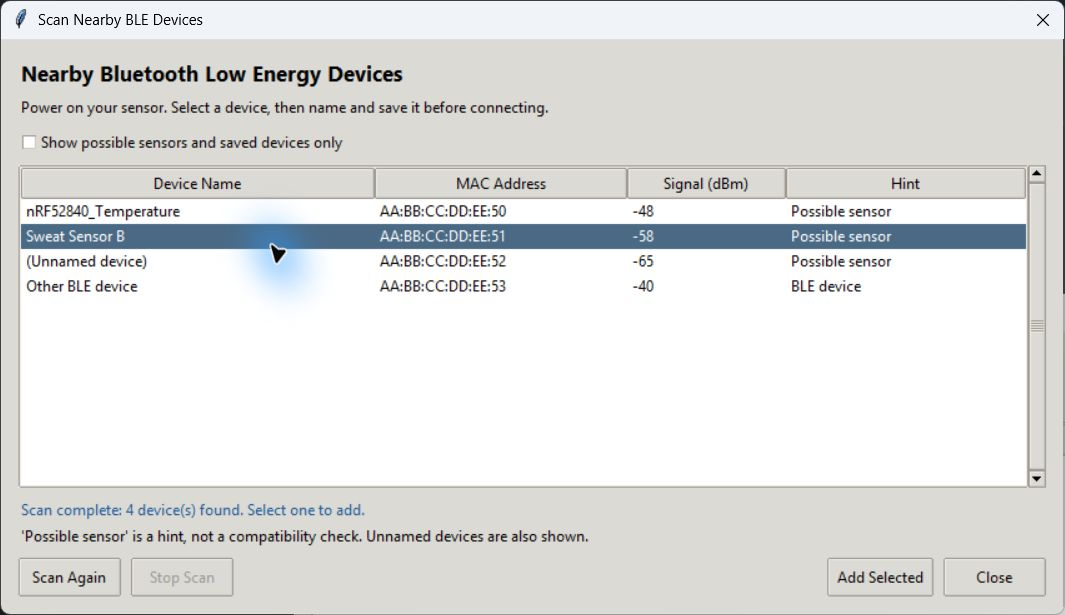
\includegraphics[width=160mm]{assets/scan.jpg}};
\framebegin
\boxat{.018}{.588}{.965}{.637}{1}
\boxat{.776}{.029}{.878}{.093}{2}
\draw[redbox,line width=.8pt] (.018,.749) rectangle (.359,.786);
\draw[redbox,line width=.8pt] (.018,.029) rectangle (.221,.093);
\frameend\end{tikzpicture}\end{center}
\vspace{-6pt}
\note{The checkbox filters to possible sensors and saved devices. ``Possible sensor'' is a name/service hint, not identity or compatibility verification. Switch on one sensor at a time; rescan with it off and then on to confirm which MAC disappears and reappears. Signal indicates signal strength. All pictured scan addresses are simulated examples.}

\vspace{3pt}
\begin{minipage}[c]{60mm}\begin{tikzpicture}
\node[anchor=south west,inner sep=0] (img) at (0,0) {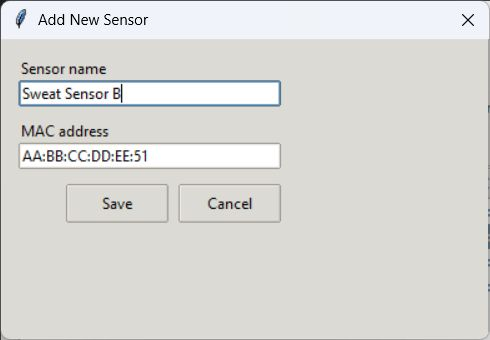
\includegraphics[width=59mm]{assets/add.jpg}};
\framebegin
\draw[redbox,line width=.8pt] (.035,.500) rectangle (.575,.765);
\boxat{.132}{.344}{.344}{.459}{3}
\frameend\end{tikzpicture}\end{minipage}\hfill
\begin{minipage}[c]{115mm}\small
\textbf{Already know the MAC?} Click \key{Add New} (A), enter a name and an address such as \texttt{AA:BB:CC:DD:EE:51}, then \key{Save}. Saved devices remain available next time.

\textbf{Multiple sensors.} Add and connect each device separately. Each has its own live window and data files. \key{Active streams} counts active acquisition tasks. An active MAC cannot be opened twice.

\textbf{Practice without hardware.} \key{Open Demo} (C) generates and saves simulated data. DEMO readings are for practice only.
\end{minipage}

\newpage
\setlength{\parskip}{3pt}
\titlespacing*{\section}{0pt}{6pt}{4pt}
{\Large\sffamily\bfseries\color{navy}Measure, mark events, and save}\hfill\note{Recording starts automatically on connection}

\section*{3\quad Apply standard solutions before measurement}
\begin{enumerate}
\item \textbf{Low point:} Apply \textbf{150 ppm standard solution} to the sensing membrane; wait for a stable curve.
\item \textbf{High point:} Apply \textbf{2000 ppm standard solution} to the sensing membrane; wait for a stable curve.
\item \textbf{After calibration:} Wear the sensor as required by your experiment and begin sweat measurement.
\end{enumerate}
\note{Adapted from the Word guide in the original archive. Follow your laboratory SOP for volume, liquid handling between solutions, and stability criteria. Record the stable voltage at each point. The software saves mV; it does not calibrate or convert to concentration. Suggested flags: blue = low point; yellow = high point.}

\section*{4\quad Read the live output and mark events}
\begin{minipage}[c]{95mm}\begin{tikzpicture}
\node[anchor=south west,inner sep=0] (img) at (0,0) {\crop{stream}{0}{855}{1470}{0}{94mm}};
\framebegin
\boxat{.022}{.245}{.300}{.580}{4}
\boxat{.022}{.070}{.850}{.235}{5}
\frameend\end{tikzpicture}\end{minipage}\hfill
\begin{minipage}[c]{79mm}\small
\textbf{4: Live readings.} \key{Last value} shows voltage; \key{Samples} increases as data arrives.

\textbf{5: File and event output.} \key{Saving to} shows the CSV filename; \key{Last flag} shows event color, time, and voltage.

Double-click the title bar to maximize the window if the bottom controls are cut off.
\end{minipage}

\begin{center}\crop{stream}{150}{165}{30}{217.5}{130mm}\end{center}
\vspace{-7pt}
\note{Plot axes: Time (s) and Voltage (mV). All screenshots use simulated devices and data for demonstration.}

\begin{minipage}[c]{113mm}\begin{tikzpicture}
\node[anchor=south west,inner sep=0] (img) at (0,0) {\crop{stream}{11.25}{48.75}{1417.5}{896.25}{112mm}};
\framebegin\boxat{.020}{.065}{.956}{.406}{6}\frameend
\end{tikzpicture}\end{minipage}\hfill
\begin{minipage}[c]{60mm}\small
\textbf{6: Mark an event.} Click a \key{Flag} button or press \key{1 / 2 / 3 / 4} in the live window for blue / yellow / red / green.
\end{minipage}
\note{Assign and document your own color meanings. A flag adds a file row and updates Last flag; it does not draw a colored event line. Receive at least one sample before adding a flag.}

\section*{5\quad Stop and find your data}
\begin{minipage}[c]{43mm}\begin{tikzpicture}
\node[anchor=south west,inner sep=0] (img) at (0,0) {\crop{stream}{1740}{3.75}{3.75}{993.75}{42mm}};
\framebegin\boxat{.038}{.140}{.506}{.910}{7}\frameend
\end{tikzpicture}\end{minipage}\hfill
\begin{minipage}[c]{131mm}\small
Click \key{Stop} (7). Wait for \key{Disconnected} and \key{Saved: ...}, then click \key{Close}. Stop each sensor separately. Closing the main window stops all streams and saves their data.
\end{minipage}

\begin{enumerate}
\item Click \key{Open Data Folder} (D) in the main window. Find the filename shown next to \key{Saving to / Saved}.
\item Each connection creates matching \textbf{CSV and TXT files}, saved continuously. No separate Save action is needed. Open either file in Excel or a text editor.
\end{enumerate}
\small Default folder: \texttt{\%LOCALAPPDATA\%\textbackslash WearableSweatSensor\textbackslash Data\textbackslash wearable device\textbackslash}

\begin{tabularx}{\linewidth}{@{}lX@{}}\toprule
\textbf{Column} & \textbf{Meaning}\\\midrule
\texttt{time\_s} & Elapsed time since this acquisition began, in seconds.\\
\texttt{voltage\_mv} & Voltage in millivolts (mV).\\
\texttt{event\_flag} & Blank for normal samples; blue / yellow / red / green for event rows.\\\bottomrule
\end{tabularx}
\note{An event row repeats the latest sample's time and voltage. Exclude rows with a nonempty event\_flag when calculating sample statistics. A failed connection may leave a header-only file; check Samples and file contents.}

\vspace{3pt}\textbf{Quick troubleshooting.} \small If no sensor appears, check its power, distance, and the computer's Bluetooth, then scan again. After an unexpected disconnect, written data remains saved; reconnecting creates new files.
\end{document}
